\documentclass[11pt]{article}
\usepackage[english]{babel}
\usepackage[utf8]{inputenc}
\usepackage[left=1cm,right=1cm,top=1cm,bottom=1.2cm]{geometry}
\usepackage{amsmath}
\usepackage{amssymb}
\usepackage{graphicx}
\usepackage{tcolorbox}
\usepackage{indentfirst}
\usepackage{hyperref}

\graphicspath{ {./images/} }

\title{\underline{IVR Coursework}}
\author{Matt Timmons-Brown \& Neil Weidinger}

\begin{document}
\maketitle

Neil and Matt worked on this coursework collaboratively - answering all questions and coding together. Thus there was an equal contribution from both members of the team.

Access the GitHub link to our code here: \url{https://github.com/the-raspberry-pi-guy/IVR-Assignment}

\setcounter{section}{1}
\section{Robot Vision}

\subsection{Joint State Estimation}
\textit{\\DESCRIBE ALGORITHM}
\begin{center}
    \begin{tabular}{ll}
        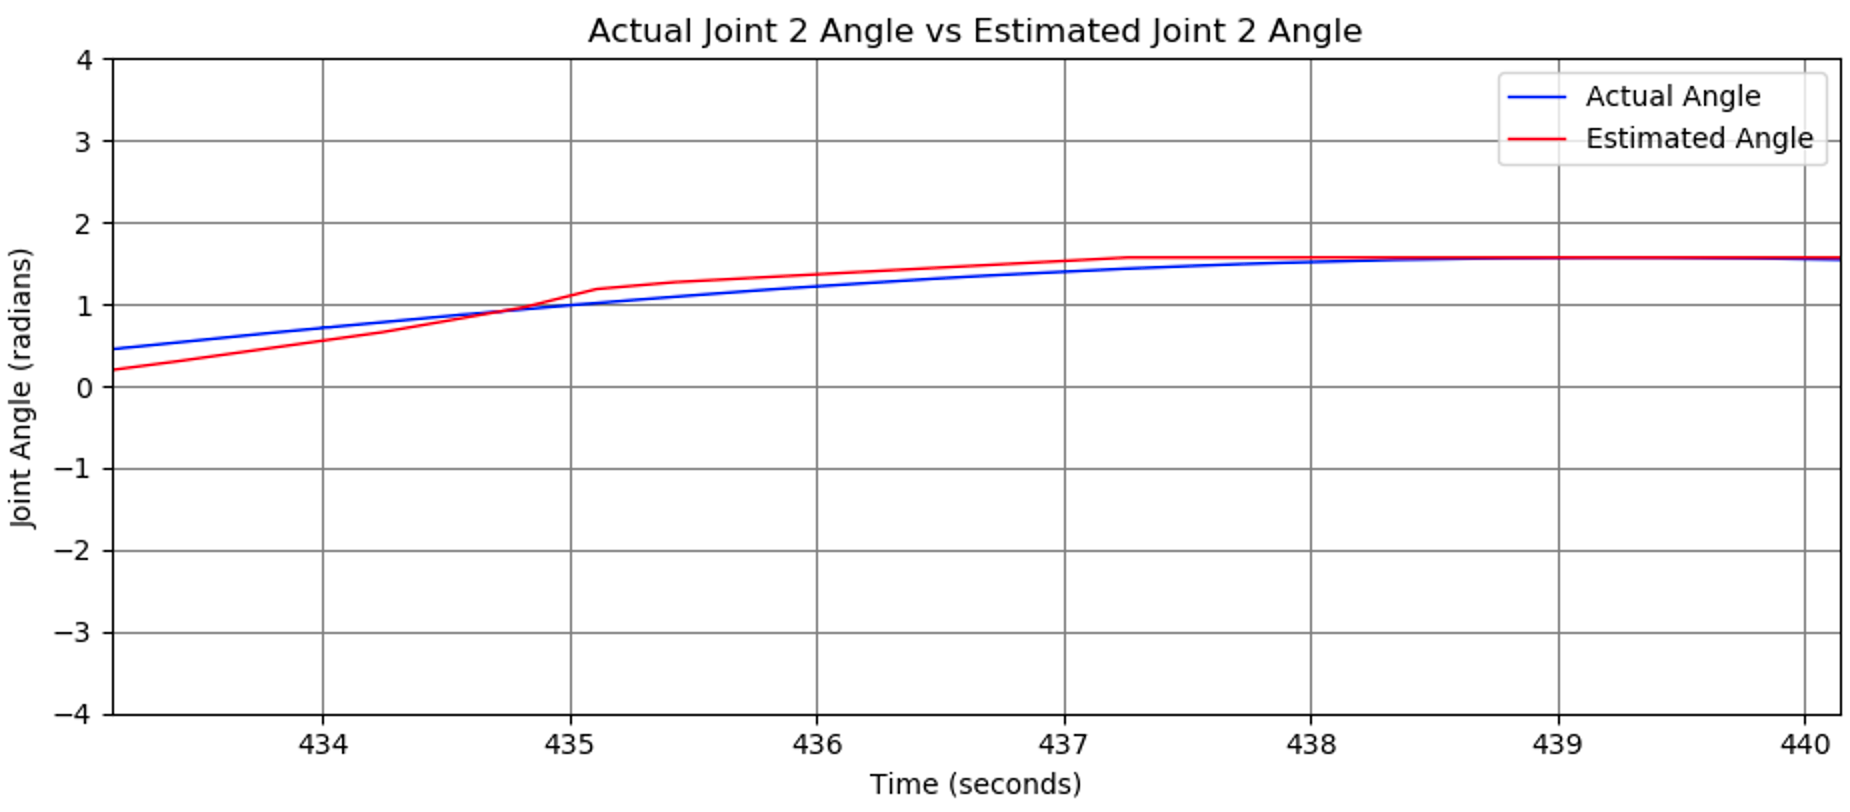
\includegraphics[width=0.4\textwidth]{images/2.1_joint2.png}
        &
        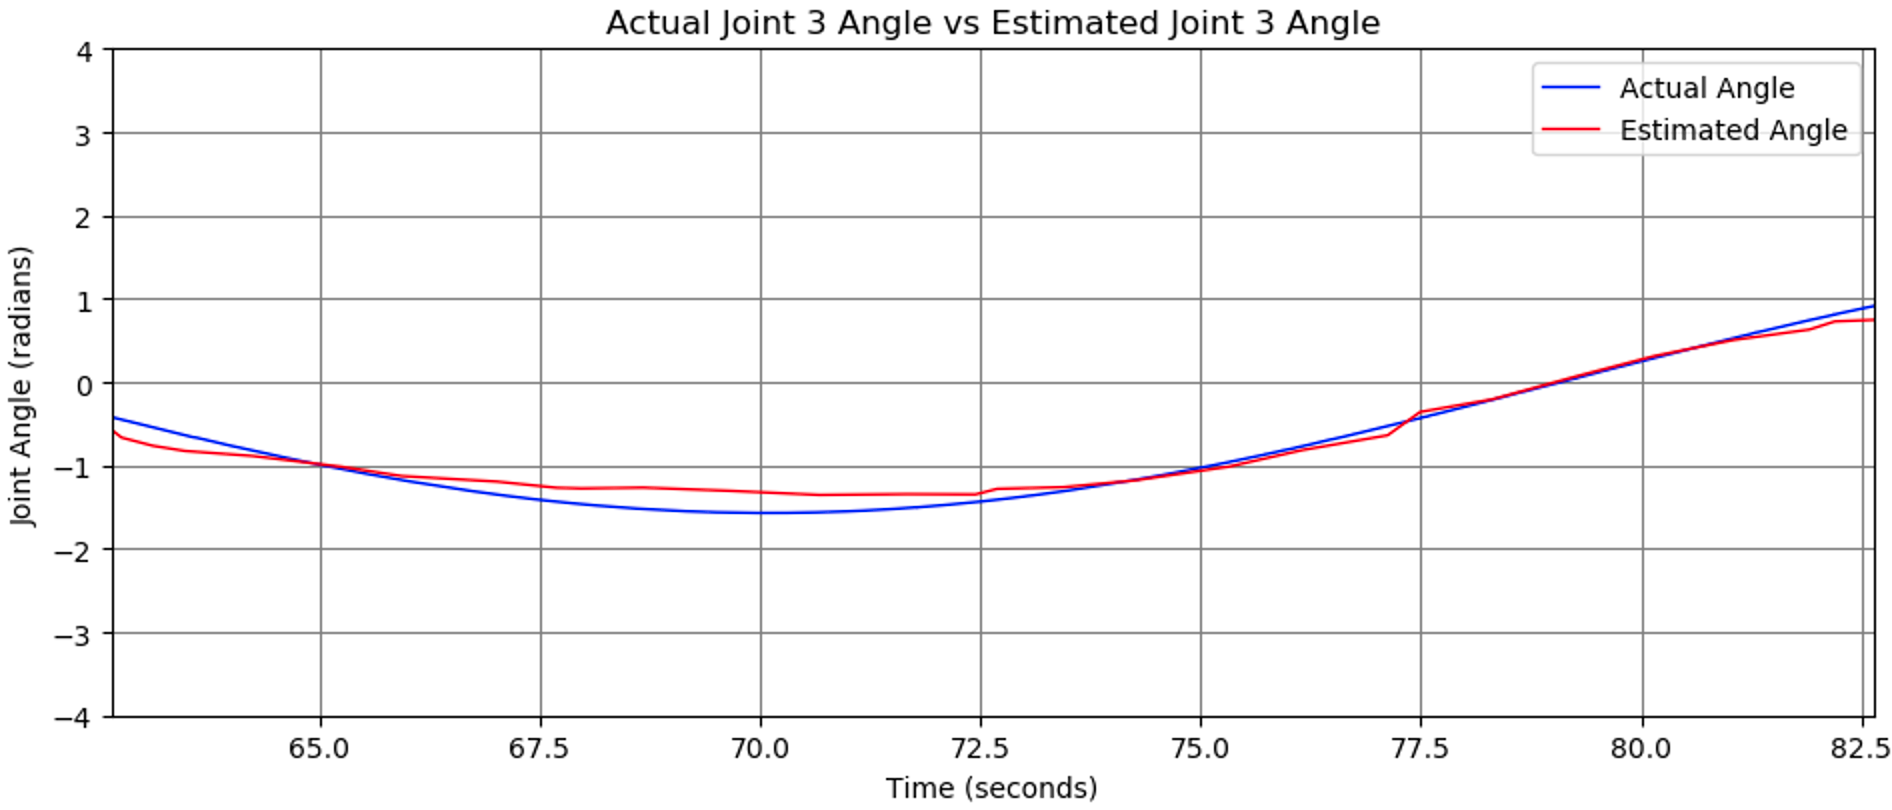
\includegraphics[width=0.4\textwidth]{images/2.1_joint3.png}
    \end{tabular}
    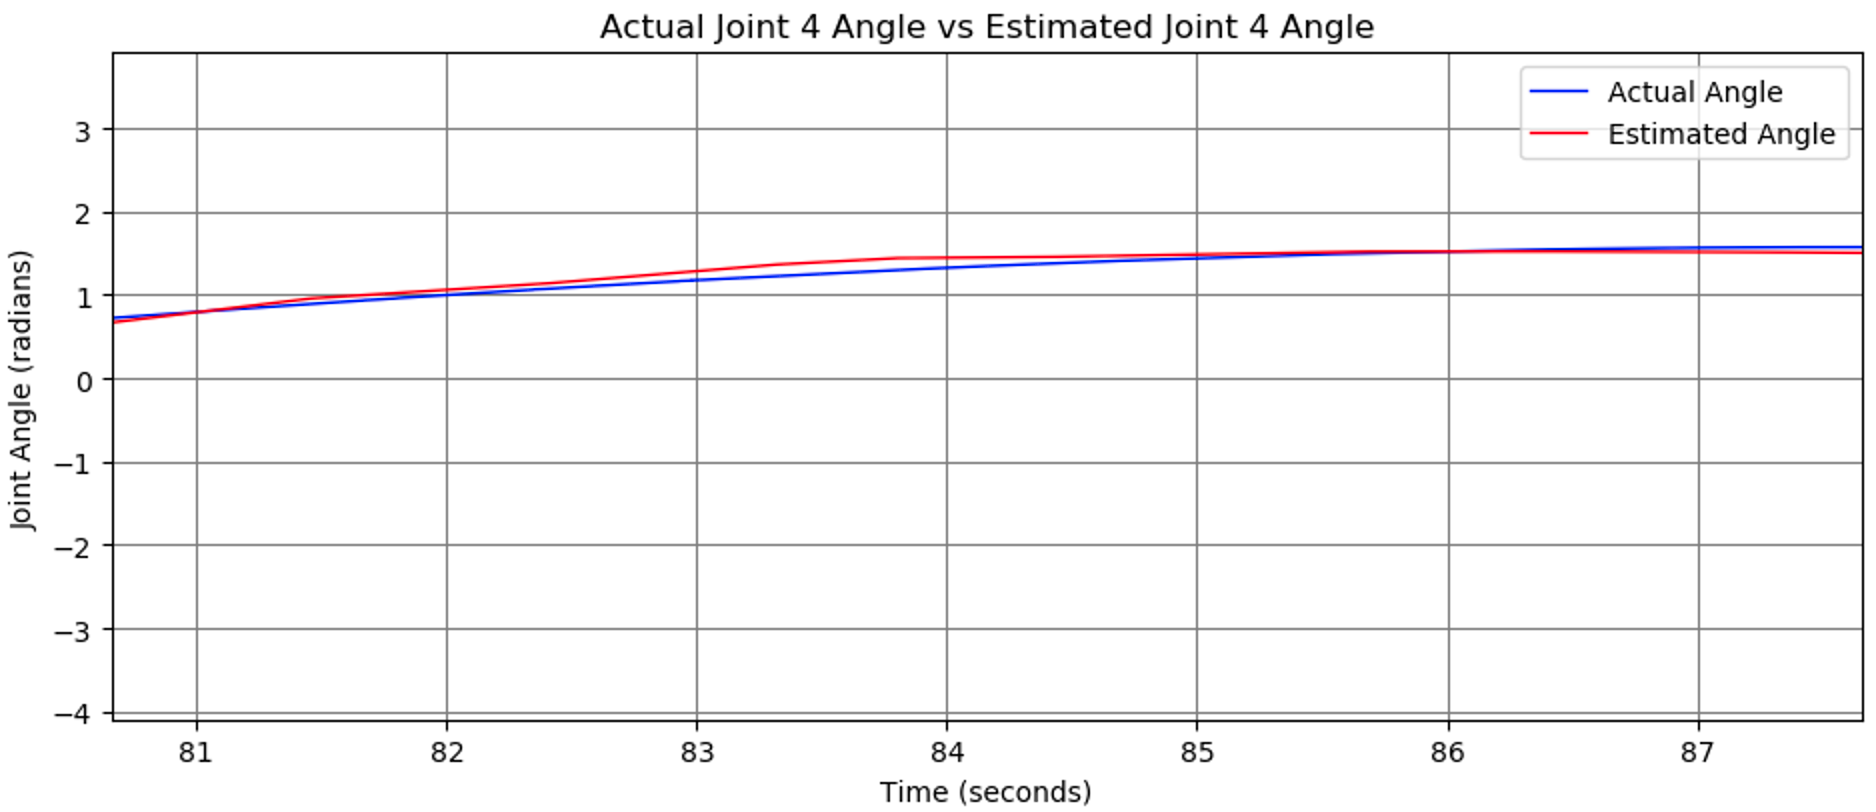
\includegraphics[width=0.4\textwidth]{images/2.1_joint4.png}
\end{center}

\subsection{Target Detection}
\textit{\\DESCRIBE ALGORITHM \& COMMENT ON SOURCES OF ERROR IN MEASUREMENTS}

\begin{center}
    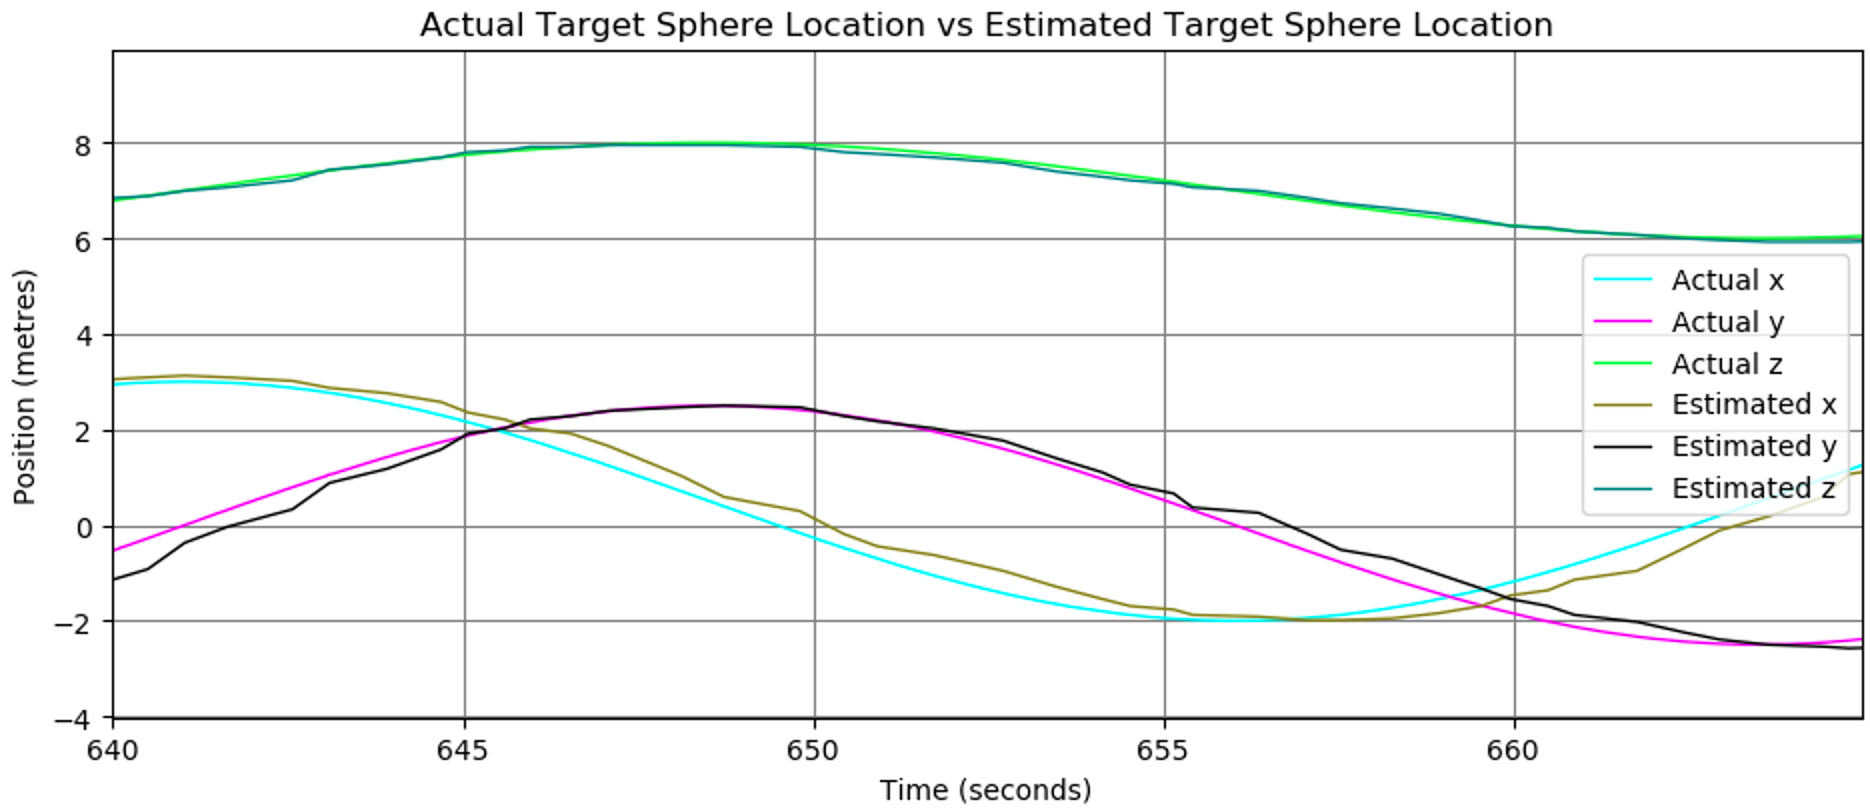
\includegraphics[width=0.4\textwidth]{images/2.2_target.png}
\end{center}

\section{Robot Control}
\subsection{Forward Kinematics}
\begin{center}
    \[\left[\begin{matrix}3 s{\left(\theta_{1} \right)} s{\left(\theta_{2} \right)} c{\left(\theta_{3} \right)} c{\left(\theta_{4} \right)} + 3.5 s{\left(\theta_{1} \right)} s{\left(\theta_{2} \right)} c{\left(\theta_{3} \right)} + 3 s{\left(\theta_{1} \right)} s{\left(\theta_{4} \right)} c{\left(\theta_{2} \right)} + 3 s{\left(\theta_{3} \right)} c{\left(\theta_{1} \right)} c{\left(\theta_{4} \right)} + 3.5 s{\left(\theta_{3} \right)} c{\left(\theta_{1} \right)}\\3 s{\left(\theta_{1} \right)} s{\left(\theta_{3} \right)} c{\left(\theta_{4} \right)} + 3.5 s{\left(\theta_{1} \right)} s{\left(\theta_{3} \right)} - 3 s{\left(\theta_{2} \right)} c{\left(\theta_{1} \right)} c{\left(\theta_{3} \right)} c{\left(\theta_{4} \right)} - 3.5 s{\left(\theta_{2} \right)} c{\left(\theta_{1} \right)} c{\left(\theta_{3} \right)} - 3 s{\left(\theta_{4} \right)} c{\left(\theta_{1} \right)} c{\left(\theta_{2} \right)}\\- 3 s{\left(\theta_{2} \right)} s{\left(\theta_{4} \right)} + 3 c{\left(\theta_{2} \right)} c{\left(\theta_{3} \right)} c{\left(\theta_{4} \right)} + 3.5 c{\left(\theta_{2} \right)} c{\left(\theta_{3} \right)} + 2.5\end{matrix}\right]\]

    \begin{tabular}{|c|c|c|}
        \hline
        Joint Angle & Estimated via FK & Estimated via Images \\
        \textit{Joint 1,2,3,4 (rad)} & \textit{x,y,z (m)} & \textit{x,y,z (m)} \\ \hline
        1,0.5,0.1,-1 & 0.47,0.31,8.18 & 0.33,0.33,8.76 \\
        -1,-1,-1,1 & -1.52,4.15,6.12 & -1.36,3.68,6.59 \\
        0.25,0.25,0.25,0.25 & 2.09, -1.79, 8.33 & 2.24,-2.06,9.16 \\
        1,1,0.5,0.5 & 6.05,-0.39,4.20 & 6.11,-0.59,4.64 \\
        -1,-0.5,-0.1,1 & 4.20,2.09,5.76 & 3.68,2.72,6.22 \\
        1,1,1,-1 & 3.14,3.10,6.12 & 2.54,3.72,6.77 \\
        -0.25,-0.25,-0.25,-0.25 & -0.98,2.58,8.33 & -0.92,2.43,8.65 \\
        -1,-1,-0.5,-0.5 & 2.88,5.34,4.20 & 2.13,6.33,4.97 \\
        \(\pi\), $\pi/2$, $\pi/4$, $-0.1$ & -4.58,4.59,2.80 & -3.72,3.64,3.86 \\
        \(-\pi\), $-\pi/2$, $-\pi/4$, $0.1$ & 4.59,-4.58,2.80 & 6.07,-6.15,2.43 \\
        \hline
    \end{tabular}
\end{center}


\textit{COMMENT ON ACCURACY}

\subsection{Closed-Loop Control}

\begin{center}
    \textbf{$A =$}
    \[\left[\begin{matrix}- 3 s{\left(\theta_{1} \right)} s{\left(\theta_{3} \right)} c{\left(\theta_{4} \right)} - 3.5 s{\left(\theta_{1} \right)} s{\left(\theta_{3} \right)} + 3 s{\left(\theta_{2} \right)} c{\left(\theta_{1} \right)} c{\left(\theta_{3} \right)} c{\left(\theta_{4} \right)} + 3.5 s{\left(\theta_{2} \right)} c{\left(\theta_{1} \right)} c{\left(\theta_{3} \right)} + 3 s{\left(\theta_{4} \right)} c{\left(\theta_{1} \right)} c{\left(\theta_{2} \right)}\\3 s{\left(\theta_{1} \right)} s{\left(\theta_{2} \right)} c{\left(\theta_{3} \right)} c{\left(\theta_{4} \right)} + 3.5 s{\left(\theta_{1} \right)} s{\left(\theta_{2} \right)} c{\left(\theta_{3} \right)} + 3 s{\left(\theta_{1} \right)} s{\left(\theta_{4} \right)} c{\left(\theta_{2} \right)} + 3 s{\left(\theta_{3} \right)} c{\left(\theta_{1} \right)} c{\left(\theta_{4} \right)} + 3.5 s{\left(\theta_{3} \right)} c{\left(\theta_{1} \right)}\\0\end{matrix}\right]\]

    \textbf{$B =$}
    \[\left[\begin{matrix}- 3 s{\left(\theta_{1} \right)} s{\left(\theta_{2} \right)} s{\left(\theta_{4} \right)} + 3 s{\left(\theta_{1} \right)} c{\left(\theta_{2} \right)} c{\left(\theta_{3} \right)} c{\left(\theta_{4} \right)} + 3.5 s{\left(\theta_{1} \right)} c{\left(\theta_{2} \right)} c{\left(\theta_{3} \right)}\\3 s{\left(\theta_{2} \right)} s{\left(\theta_{4} \right)} c{\left(\theta_{1} \right)} - 3 c{\left(\theta_{1} \right)} c{\left(\theta_{2} \right)} c{\left(\theta_{3} \right)} c{\left(\theta_{4} \right)} - 3.5 c{\left(\theta_{1} \right)} c{\left(\theta_{2} \right)} c{\left(\theta_{3} \right)}\\- 3 s{\left(\theta_{2} \right)} c{\left(\theta_{3} \right)} c{\left(\theta_{4} \right)} - 3.5 s{\left(\theta_{2} \right)} c{\left(\theta_{3} \right)} - 3 s{\left(\theta_{4} \right)} c{\left(\theta_{2} \right)}\end{matrix}\right]\]

    \textbf{$C =$}
    \[\left[\begin{matrix}- 3 s{\left(\theta_{1} \right)} s{\left(\theta_{2} \right)} s{\left(\theta_{3} \right)} c{\left(\theta_{4} \right)} - 3.5 s{\left(\theta_{1} \right)} s{\left(\theta_{2} \right)} s{\left(\theta_{3} \right)} + 3 c{\left(\theta_{1} \right)} c{\left(\theta_{3} \right)} c{\left(\theta_{4} \right)} + 3.5 c{\left(\theta_{1} \right)} c{\left(\theta_{3} \right)}\\3 s{\left(\theta_{1} \right)} c{\left(\theta_{3} \right)} c{\left(\theta_{4} \right)} + 3.5 s{\left(\theta_{1} \right)} c{\left(\theta_{3} \right)} + 3 s{\left(\theta_{2} \right)} s{\left(\theta_{3} \right)} c{\left(\theta_{1} \right)} c{\left(\theta_{4} \right)} + 3.5 s{\left(\theta_{2} \right)} s{\left(\theta_{3} \right)} c{\left(\theta_{1} \right)}\\- 3 s{\left(\theta_{3} \right)} c{\left(\theta_{2} \right)} c{\left(\theta_{4} \right)} - 3.5 s{\left(\theta_{3} \right)} c{\left(\theta_{2} \right)}\end{matrix}\right]\]

    \textbf{$D =$}
    \[\left[\begin{matrix}- 3 s{\left(\theta_{1} \right)} s{\left(\theta_{2} \right)} s{\left(\theta_{4} \right)} c{\left(\theta_{3} \right)} + 3 s{\left(\theta_{1} \right)} c{\left(\theta_{2} \right)} c{\left(\theta_{4} \right)} - 3 s{\left(\theta_{3} \right)} s{\left(\theta_{4} \right)} c{\left(\theta_{1} \right)}\\- 3 s{\left(\theta_{1} \right)} s{\left(\theta_{3} \right)} s{\left(\theta_{4} \right)} + 3 s{\left(\theta_{2} \right)} s{\left(\theta_{4} \right)} c{\left(\theta_{1} \right)} c{\left(\theta_{3} \right)} - 3 c{\left(\theta_{1} \right)} c{\left(\theta_{2} \right)} c{\left(\theta_{4} \right)}\\- 3 s{\left(\theta_{2} \right)} c{\left(\theta_{4} \right)} - 3 s{\left(\theta_{4} \right)} c{\left(\theta_{2} \right)} c{\left(\theta_{3} \right)}\end{matrix}\right]\]
\end{center}
Where A, B, C and D are column vectors that form the Jacobian when arranged like (formatted to save space):
\[\left[\begin{matrix} A & B & C & D \end{matrix}\right]\]

\textit{\\PRESENT THREE PLOTS COMPARING THE X,Y,Z POSITION OF THE ROBOT END-EFFECTOR WITH THE X,Y,Z POSITION OF THE TARGET FOR 10 SECONDS.}

\section{Final Task}
\setcounter{subsection}{1}
\subsection{Null-space Control}

\textit{\\DISCUSS ALGORITHM AND HOW IT IS DIFFERENT FROM PREVIOUS CONTROLLER. THREE PLOTS COMPARING THE POSITION OF THE ROBOT END-EFFECTOR WITH THE POSITION OF THE SPHERE AND THE POSITION OF THE BOX.}

\end{document}